\chapter{Introdução}

%=====================================================

Estima-se que em 2020 já existiam cerca de 40.000 \emph{exabytes} de dados digitalizados no mundo, e uma fração de 33\% destes dados podem ser valiosos depois de analisados \cite{gantz2012digital}. Construir \emph{clusters} com capacidade de armazenar e processar essa enorme quantidade de dados para extrair informações úteis às empresas tem-se tornado um enorme desafio, principalmente devido ao ritmo de crescimento exponencial deste volume de dados.

Nas últimas duas décadas o Hadoop, uma plataforma de código fonte aberto mantida pela Apache Software Foundation para criar e gerenciar Infraestruturas de \emph{clusters} baseados em \emph{MapReduce} tem se destacado. A principal motivação para uso do Hadoop é sua escalabilidade, que permite unificar várias máquinas convencionais gerando grandes capacidades de armazenamento e processamento em massa de dados estruturados e, principalmente, não estruturados \cite{goldman2012apache}.

Atualmente servidores com Hadoop tem sido oferecido no mercado por multinacionais como Amazon, Microsoft, Google, entre outras. Estes serviços fazem parte da computação em nuvem e utilizam conexões Ethernet para trocas de informações (tráfego) entre \emph{clusters}, e consequentemente, aumentam o consumo de energia nos \emph{Data  Centers}. Tráfegos de dados gerados nas comunicações entre \emph{clusters} em empresas privadas também são contabilizados como tráfego da computação em nuvem pela Cisco \cite{cisco2020cisco}.

Embora seu conceito tenha surgido em 1960, a computação em nuvem só ganhou forma no século XXI devido à indisponibilidade de recursos para implementá-la de fato. Computação em nuvem é um termo utilizado para descrever o ambiente de computação baseado em uma imensa rede de servidores virtuais e físicos, que geram um conjunto de recursos com capacidade de processamento, armazenamento, conectividade, plataformas, aplicações e serviços disponibilizados na Internet \cite {taurion2009cloud}. Dentre suas principais características pode-se notar:

\begin{itemize}
\item A sensação de possuir recursos infinitos disponibilizados sob demanda do usuário;
\item Elimina a necessidade de adquirir recursos antecipadamente, como por exemplo, servidores para implementar negócios;
\item Disponibilidade elástica de recursos, permitindo que os usuários usem os recursos na quantidade que forem necessários, aumentando e diminuindo a capacidade computacional de forma dinâmica;
\item O pagamento final se dá somente pela quantidade de recursos computacionais utilizados (\emph{pay-per-use}).
\end{itemize}

No início dos anos 2000, multinacionais como Google e Amazon começaram a criar imensos parques computacionais baseados no conceito de computação em nuvem para operarem seus negócios, e logo adiante outras seguiram seus exemplos, como a IBM, Intel, Apple, Microsoft, Yahoo, Apache Software Foundation, Ask, entre outras \cite {taurion2009cloud}.

A Cisco vem publicando artigos nos últimos anos que demonstram o impacto deste investimento e desenvolvimento de tecnologias no tráfego de dados em nuvem. Em 2013 o tráfego de \emph{Cloud Data Centers} já representava cerca de 54\% de todo o tráfego em \emph{Data Centers} globais \cite {index2014forecast}. A partir daí só continuou a aumentar, em 2018 já eram 76\%, em 2020 cerca de 92\%, e em 2021 foi de aproximadamente 95\% \cite {index2018forecast}.

\begin{figure}[htp]
    \centering
    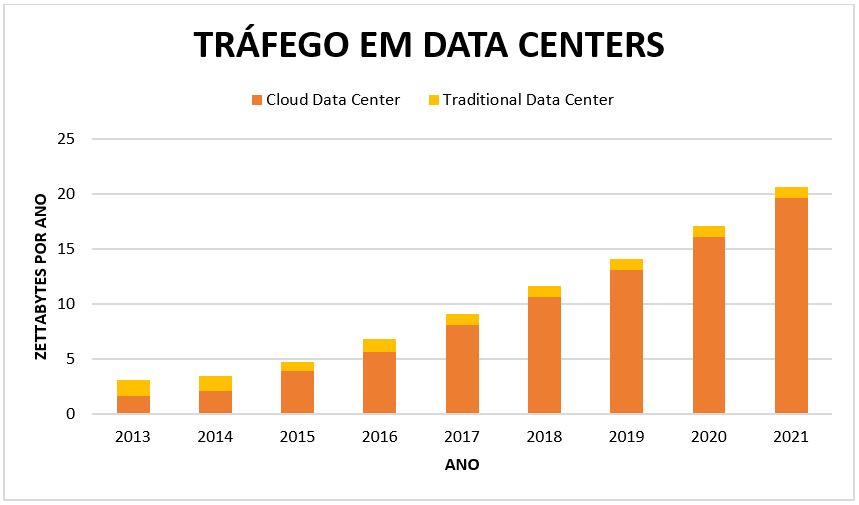
\includegraphics[width=12cm]{1-intro/Figura_1.jpg}
    \caption{Tráfego em Data Centers estimado pela Cisco}
    \cite {index2018forecast}
    \label{fig:trafegoestimado}
\end{figure}

Como esperado, a previsão de 2018 \cite{index2018forecast} superou a anterior de 2014 \cite{index2014forecast}, isso se deve ao fato de a \emph{Cloud Computing} estar sendo implantada no cotidiano das organizações mais rápido do que se esperava. Na figura 1.1 pode-se observar o tráfego de dados em \emph{Data Centers}, incluindo 2021.

Além disso, outras informações são notáveis, como o detalhamento das formas de tráfego de dados que acontecem nas \emph{Cloud Data Centers}. Pode-se classificá-las de três maneiras:

\begin{itemize}
\item Tráfego de \emph{Data Center} para Usuário: Este tráfego é gerado quando usuários utilizam serviços de E-mail e \emph{Video-on-demand} (VOD).
\item Tráfego de \emph{Data Center} para \emph{Data Center}: O tráfego entre \emph{data centers} é gerado por tarefas como replicação de arquivos (comuns no \emph{Hadoop Distributed File System}), \emph{Content Delivery Networks} (CDN) e enlaces entre nuvens que enviam e recebem informações sobre o armazenamento e processamento de dados em cada \emph{Data Center}, entre outros.
\item Tráfego Interno no \emph{Data Center}: Também conhecido como Tráfego Leste-Oeste, consiste em dados de armazenamento, processamento (principalmente os massivos de \emph{Big Data}), desenvolvimento, entres outras.
\end{itemize}

Pode-se observar na figura 1.2 a quantia de tráfego em cada uma das categorias nos últimos seis anos em \emph{Zettabytes}. Com essas informações conclui-se que o tráfego gerado pelo processamento de dados dentro dos \emph{Data Centers} tem sido o principal motivo deste aumento gigantesco.

\begin{figure}[htp]
    \centering
    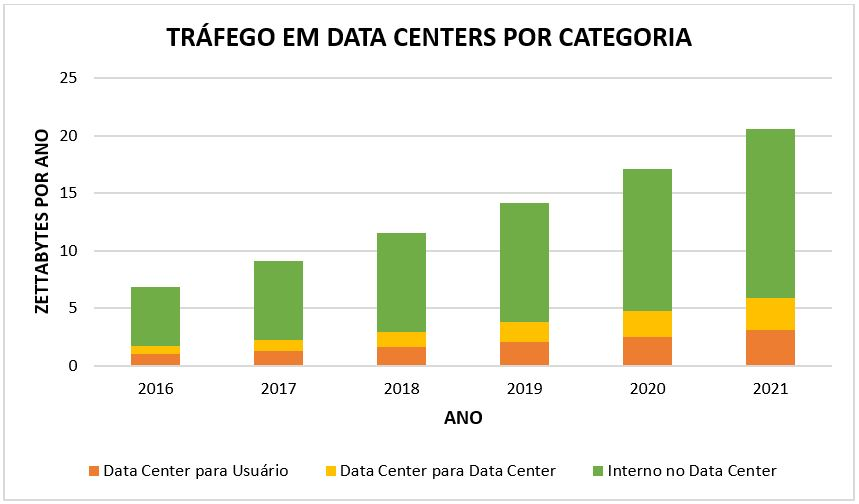
\includegraphics[width=12cm]{1-intro/Figura_2.jpg}
    \caption{Tráfego em Data Centers por Categoria estimado pela Cisco}
    \cite{index2018forecast}
    \label{fig:trafegoestimadoporcategoria}
\end{figure}

O tráfego que permanece nos \emph{data centers} diminuiu ligeiramente até 2021, de 75,4\% para 71,5\%. Entretanto, estes dados não incluem as métricas de tráfegos locais dos racks (intra-racks). Caso fossem incluídas, a previsão é que o tráfego residente nos \emph{data centers} atingiria mais de 90\%. A \emph{Big Data} possui uma porcentagem extremamente significativa no tráfego dentro dos \emph{data centers}. Embora grande parte dos processamentos desta área seja intra-rack, ainda assim, o tráfego de um rack para outro foi o suficiente para ser responsável por pelo menos 20\% de todo o tráfego global entre \emph{data centers} em 2021  \cite{index2018forecast}.

No geral, o tráfego leste-oeste (tráfego interno nos \emph{data centers} e entre os \emph{data centers}) representou 85,10\% do total em 2021, e o tráfego norte-sul (tráfego saindo dos data centers para a Internet ou WAN) foi de apenas 14,90\% do tráfego associado a \emph{data centers}. Pode-se observar estas informações detalhadamente na figura 1.3, que demonstram o crescimento anual dos tráfegos em \emph{data centers} até 2021 \cite{index2018forecast}.

\begin{figure}[!htb]
    \centering
    \label{fig:subfig}
    \subfloat[Taxa de Crescimento Anual Composta \label{fig:taxacomposta}]{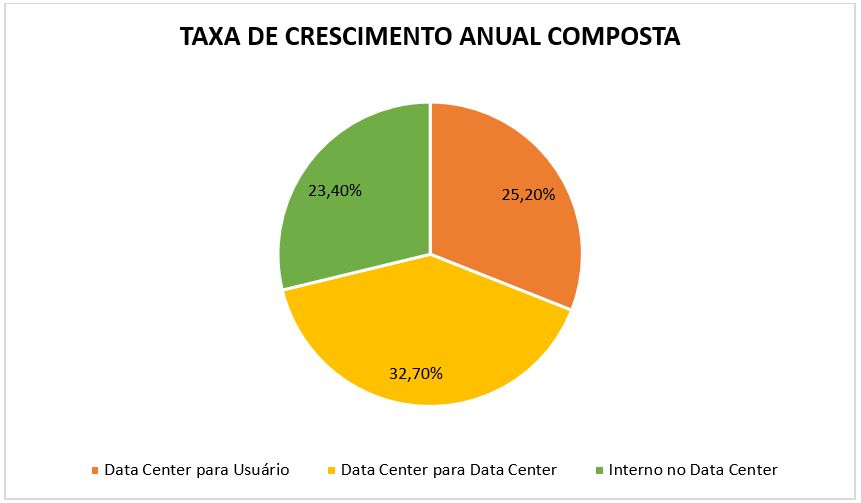
\includegraphics[width=8cm]{1-intro/Figura_3.jpg}}\hfill
    \subfloat[Tráfego Estimado em 2021
    \label{fig:trafegoestimado2021}]{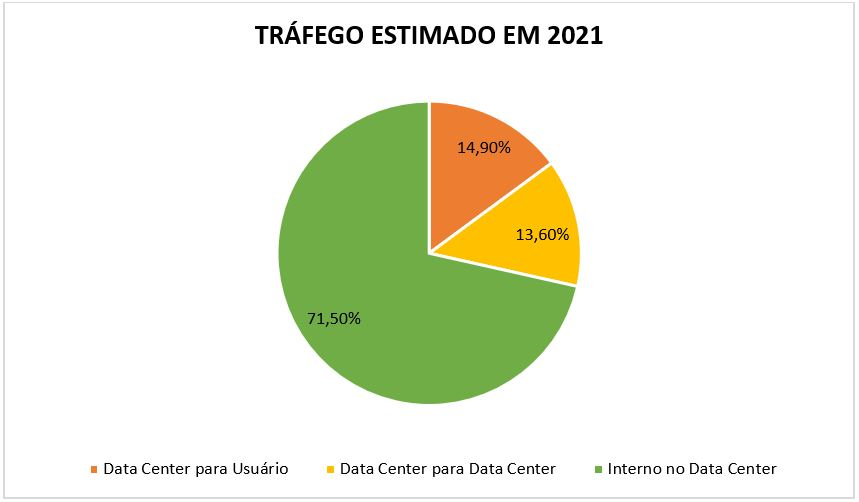
\includegraphics[width=8cm]{1-intro/Figura_4.jpg}}
    \caption{Previsões de Tráfegos para 2021 de acordo com a Cisco}
    \cite{index2018forecast}
\end{figure}

Consequentemente este enorme tráfego de dados gera um dos principais problemas nos \emph{data centers} atuais, o consumo de energia, que chega facilmente na casa de bilhões de kWh consumidos por ano \cite{raizada2020worldwide}. Este é o caso dos \emph{Data Centers} do Estados Unidos que em 2021 consumiram aproximadamente 73 bilhões de kWh \cite{shehabi2016united}. Um relatório da EPA aponta que de toda a energia consumida no mundo em 2010, cerca de 1,3\% foram em \emph{Data Centers} \cite{koomey2011growth}. Outra pesquisa ainda indica que esse consumo chegue a 3000 bilhões de kWh em 2030 \cite{raizada2020worldwide}.

De acordo com \cite{belady2007data} os custos energéticos dos \emph{Data Centers} seriam maiores que o valor gasto com as infraestruturas (\emph{hardware}) em 2008, e em 2014 este valor já seria responsável por mais de 75\% de todo o valor investido, que envolve gastos com energia, infraestrutura, funcionários e manutenção.

Em média 10\% a 50\% do consumo de energia dos \emph{Data Centers} são por DCNs - \emph{Data Center Networks} \cite{abts2010energy}, e este número tende a tornar-se maior quando os recursos não são utilizados totalmente por uma execução. De toda a energia utilizada nos \emph{clusters}, cerca de 30\% são consumidas por \emph{switches}  \cite{kliazovich2012greencloud}.

Conforme relatado em \cite{mahadevan2009energy} é possível diminuir este consumo de energia, uma vez que os \emph{links} de interconexão que são responsáveis por 65\% do consumo de energia total dos \emph{switches}, não cessam o consumo total mesmo quando não estão sendo utilizados pelo \emph{data center} \cite{christensen2010ieee}.

\emph{Clusters} Hadoop possuem comunicações complexas que utilizam \emph{links} de interconexão com frequência, principalmente nas fases \emph{Shuffle} e \emph{Reduce} de uma aplicação \emph{MapReduce}, em que todos os nodos do aglomerado se comunicam entre si \cite{dean2004mapreduce}.

O padrão Energy Efficient Ethernet (EEE) visa reduzir o consumo de energia das conexões Ethernet, definindo um modo de hibernação de link conhecido como \emph{Low Power Idle}. Inicialmente o EEE foi desenvolvido para pequenos ambientes, como pequenas empresas e escritórios domésticos, e posteriormente para aplicações de \emph{big data} de \emph{data centers}, incluindo streaming de vídeo e \emph{data science}. Como o EEE pode causar sobrecarga de rede e perda de desempenho, muitos fornecedores de equipamentos aconselham seus clientes a desativá-lo em uso de produção. No entanto, estudos recentes apontam que o EEE pode ser habilitado em ambientes de produção \emph{MapReduce} se configurado corretamente \cite{e2015exploring} \cite{e2017energy}.

O estudo mais importante que demonstra a eficácia do EEE em \emph{clusters} Hadoop pode ser encontrado em E-EON - \emph{Energy-Efficient and Optimized Networks for Hadoop} \cite{silva2018eon}. Recentemente, foi demonstrado como obter alto desempenho em \emph{clusters} Hadoop com o EEE habilitado para links de 1GbE e 10GbE. Nesta pesquisa é apresentado um conjunto de técnicas que podem ser utilizadas para reduzir o consumo de energia da rede e diminuir ainda mais a latência, enquanto melhora a taxa de transferência do cluster Hadoop. Além disso, essas técnicas não são exclusivas do Hadoop e pode-se obter benefícios semelhantes se aplicadas a qualquer outra carga de trabalho que seja semelhante em funcionamento ao \emph{MapReduce}.

%\section{Proposta e Desafios}

\section{Objetivos e Contribuições}

Conforme a demanda de energia por \emph{Data Centers} Hadoop aumentam torna-se necessária a otimização e redução do consumo. O principal objetivo da nossa pesquisa é avaliar o consumo de energia da atual versão do Hadoop \emph{MapReduce} (3.x) através da implementação do EEE nas conexões, para isso, os seguintes objetivos específicos foram considerados:

\begin{enumerate}

\item Analisar de forma geral como a versão atual do Apache Hadoop (3.x) se comporta quando o EEE está habilitado para conexões de 1GbE e 10GbE no \emph{cluster MapReduce};

\item Realizar um estudo experimental para descobrir o potencial de economia de energia nos clusters Hadoop \emph{MapReduce} se o EEE for implementado para conexões 25GbE, 40GbE, 100GbE e 400GbE.

\end{enumerate}

Ainda como objetivos secundários, pretendemos responder algumas questões que permanecem sem respostas exatas até o presente momento:

\begin{itemize}

    \item Como estas configurações de fato afetam o funcionamento de uma execução completa de um processamento no Hadoop \emph{MapReduce}?
    
    \item Estas configurações afetam a versão 3.x da mesma forma que a versão 2.x e 1.x, ou há diferenças?
    
\end{itemize}

\section{Estrutura da Dissertação}

Esta dissertação está dividida em 6 capítulos, incluindo a Introdução como o primeiro Capítulo. No Capítulo 2 está a Fundamentação Teórica. Neste capítulo são explorados os conceitos abordados nesta pesquisa, como \emph{Ethernet Energy Efficient}, \emph{Packet Coalescing}, \emph{Random Early Detection}, \emph{Controlled Delay}, \emph{Explicit Congestion Notification}, \emph{MapReduce} e Hadoop.

O Capítulo 3 contém a Metodologia, em que é apresentada de forma completa o NetSLS, uma extensão do \emph{YARN Scheduler Load Simulator}, que nos permite realizar simulações de \emph{clusters} Hadoop, observar o consumo de recursos em tempo real através de gráficos, além de uma visão ampla da execução com rastreamentos em \emph{logs}, e assim calcular a economia de energia e desempenho. No mesmo capítulo é definida as configurações das tecnologias \emph{Ethernet Energy Efficient}, \emph{Packet Coalescing}, \emph{Random Early Detection}, \emph{Controlled Delay}, \emph{Explicit Congestion Notification}, as cargas de trabalhos \emph{small tasks} e \emph{batch}, e um ciclo de testes.

Em seguida, no Capítulo 4, é apresentada uma visão geral de como a versão atual do Apache Hadoop (3.x) se comporta quando o EEE está habilitado para links de 1GbE e 10GbE no cluster, além de uma demonstração do potencial de economia de energia em \emph{clusters Hadoop MapReduce} se o EEE estiver habilitado para links de 25GbE, 40GbE, 100GbE e 400GbE.

No Capítulo 5 são tratados os problemas das conexões acima de 40GbE, as quais possuem uma grande perda de desempenho quando o EEE está habilitado. Para isso, foram combinados \emph{Ethernet Energy Efficient} com \emph{Packet Coalescing}, \emph{Random Early Detection}, \emph{Controlled Delay} e \emph{Explicit Congestion Notification}, chegando assim à uma ótima economia de energia com perda de desempenho relativamente baixa. Ainda no Capítulo 5, comparamos nosso trabalho com o E-EON - uma série de configurações para se obter alto desempenho em \emph{clusters} Hadoop com o EEE habilitado para links de 1 GbE e 10 GbE. Por fim, o Capítulo 6 apresenta as Considerações Finais e os Trabalhos Futuros desta pesquisa.

%=====================================================
